\documentclass[12pt]{Qual}
\usepackage{preamble}

\name{Kayla Orlinsky}
\course{Complex Analysis Exam}
\term{Spring 2010}
\hwnum{Spring 2010}

\begin{document}

\begin{problem} $\,$
Map the region $\Omega=\{\im(z)>0\}\backslash\{iy\,|\,0<y\le 1\}$ conformally to the unit disk $D=\{|z|<1\}$.
\end{problem}


\begin{solution}$\,$
The issue is that $\Omega$ is missing a line segment. To remove this, we must shrink and expand the region to fill in the missing line segment.

Let \begin{align*}
    T(z)&=\frac{z-i}{z+i}\\
    w_1(z)&=z^\frac{1}{2}\qquad\text{branch at }(-\infty,0]\\
    w_2(z)&=-iz\\
    w_3(z)&=z^2
\end{align*}

Then,

\begin{center}
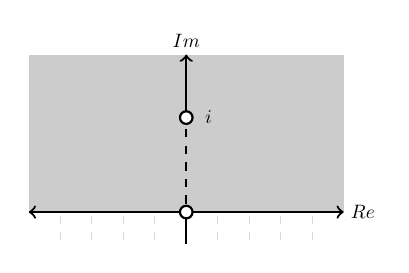
\begin{tikzpicture}[thick,scale=0.4, every node/.style={scale=0.7}]
\draw[help lines, color=gray!30, dashed] (-4.9,-0.9) grid (4.9,4.9);
 \fill[gray!40,even odd rule] (-5,0) rectangle (5,5);
\draw[<->, thick] (-5,0)--(5,0) node[right]{$Re$};
\draw[->, thick] (0,-1)--(0,5) node[above]{$Im$};
\draw[gray!40, line width=0.5mm, dashed] (0,0)--(0,3) node[black,right,xshift=0.2cm,]{$i$};
 \filldraw[white, draw=black] (0,0) circle (0.2cm);
 \filldraw[white, draw=black] (0,3) circle (0.2cm);
\end{tikzpicture}
\begin{tikzpicture}
\draw[color=white] (-1,0) rectangle (0.5,1);
\draw[thick,->] (-1,2) -- (0,2) node[above,xshift=-0.5cm]{$T$};
\end{tikzpicture}
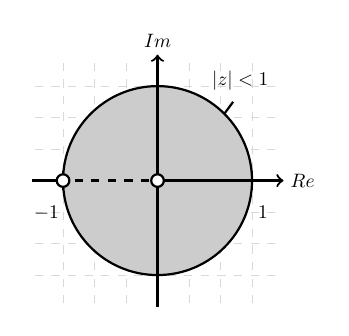
\begin{tikzpicture}[thick,scale=0.4, every node/.style={scale=0.7}]
\draw[help lines, color=gray!30, dashed] (-3.9,-3.9) grid (3.9,3.9);
\draw (2.12,2.12) -- (2.4,2.5);
 \fill[gray!40,even odd rule, dashed] (0,0) circle (3cm);
   \draw (0, 0) circle (3cm) node[above,xshift=1.5cm,yshift=1.5cm]{$|z|<1$};
\draw[thick] (3,-0.3) -- (3,0.3) node[below,xshift=0.2cm,yshift=-0.5cm]{$1$};
\draw[->, thick] (-4,0)--(4,0) node[right]{$Re$};
\draw[->, thick] (0,-4)--(0,4) node[above]{$Im$};
\draw[thick] (-3,-0.3) -- (-3,0.3) node[below,xshift=-0.3cm,yshift=-0.5cm]{$-1$};
\draw[gray!40, line width=0.5mm, dashed] (0,0)--(-3,0);
 \filldraw[white, draw=black] (0,0) circle (0.2cm);
 \filldraw[white, draw=black] (-3,0) circle (0.2cm);
\end{tikzpicture}
\begin{tikzpicture}
\draw[color=white] (-1,0) rectangle (0.5,1);
\draw[thick,->] (-1,2) -- (0,2) node[above,xshift=-0.5cm]{$w_1$};
\end{tikzpicture}
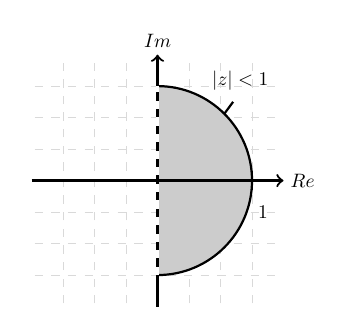
\begin{tikzpicture}[thick,scale=0.4, every node/.style={scale=0.7}]
\draw[help lines, color=gray!30, dashed] (-3.9,-3.9) grid (3.9,3.9);
\draw (2.12,2.12) -- (2.4,2.5);
 \fill[gray!40,even odd rule, dashed] (0,0) circle (3cm);
   \draw (0, 0) circle (3cm) node[above,xshift=1.5cm,yshift=1.5cm]{$|z|<1$};
\draw[thick] (3,-0.3) -- (3,0.3) node[below,xshift=0.2cm,yshift=-0.5cm]{$1$};
\draw[thick] (-3,-0.3) -- (-3,0.3) node[below,xshift=-0.3cm,yshift=-0.5cm]{$-1$};
\fill[white] (-4,-4) rectangle (0,4);
\draw[help lines, color=gray!30, dashed] (-3.9,-3.9) grid (0,3.9);
\draw[->, thick] (-4,0)--(4,0) node[right]{$Re$};
\draw[->, thick] (0,-4)--(0,4) node[above]{$Im$};
\draw[white,line width=0.4mm, dashed] (0,-3)--(0,3);
\end{tikzpicture}

\begin{tikzpicture}%[thick,scale=0.5, every node/.style={scale=0.6}]
\draw[thick,->] plot [smooth] coordinates {(3,0.6) (3,0) (-10,0) (-11,-1)} node[above,xshift=7cm,yshift=1cm]{$w_2$};
\end{tikzpicture}

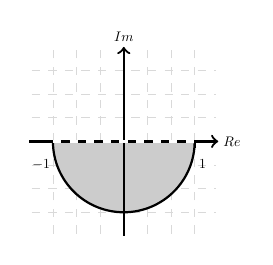
\begin{tikzpicture}[thick,scale=0.3, every node/.style={scale=0.5}]
\draw[help lines, color=gray!30, dashed] (-3.9,-3.9) grid (3.9,3.9);
\draw (2.12,2.12) -- (2.4,2.5);
 \fill[gray!40,even odd rule, dashed] (0,0) circle (3cm);
   \draw (0, 0) circle (3cm);
\draw[thick] (3,-0.3) -- (3,0.3) node[below,xshift=0.2cm,yshift=-0.5cm]{$1$};
\draw[thick] (-3,-0.3) -- (-3,0.3) node[below,xshift=-0.3cm,yshift=-0.5cm]{$-1$};
\fill[white] (-4,4) rectangle (4,0);
\draw[help lines, color=gray!30, dashed] (-3.9,3.9) grid (3.9,0);
\draw[->, thick] (-4,0)--(4,0) node[right]{$Re$};
\draw[->, thick] (0,-4)--(0,4) node[above]{$Im$};
\draw[white,line width=0.4mm, dashed] (-3,0)--(3,0);
\end{tikzpicture}
\begin{tikzpicture}
\draw[color=white] (-1,0) rectangle (0.5,1);
\draw[thick,->] (-1,2) -- (0,2) node[above,xshift=-0.5cm]{$T^{-1}$};
\end{tikzpicture}
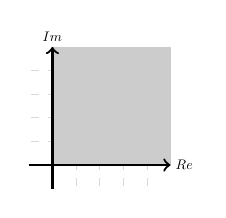
\begin{tikzpicture}[thick,scale=0.3, every node/.style={scale=0.5}]
\draw[help lines, color=gray!30, dashed] (-0.9,-0.9) grid (4.9,4.9);
 \fill[gray!40,even odd rule] (0,0) rectangle (5,5);
\draw[->, thick] (-1,0)--(5,0) node[right]{$Re$};
\draw[->, thick] (0,-1)--(0,5) node[above]{$Im$};
\end{tikzpicture}
\begin{tikzpicture}
\draw[color=white] (-1,0) rectangle (0.5,1);
\draw[thick,->] (-1,2) -- (0,2) node[above,xshift=-0.5cm]{$w_3$};
\end{tikzpicture}
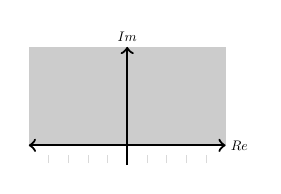
\begin{tikzpicture}[thick,scale=0.25, every node/.style={scale=0.5}]
\draw[help lines, color=gray!30, dashed] (-4.9,-0.9) grid (4.9,4.9);
 \fill[gray!40,even odd rule] (-5,0) rectangle (5,5);
\draw[<->, thick] (-5,0)--(5,0) node[right]{$Re$};
\draw[->, thick] (0,-1)--(0,5) node[above]{$Im$};
\end{tikzpicture}
\begin{tikzpicture}
\draw[color=white] (-1,0) rectangle (0.5,1);
\draw[thick,->] (-1,2) -- (0,2) node[above,xshift=-0.5cm]{$T$};
\end{tikzpicture}
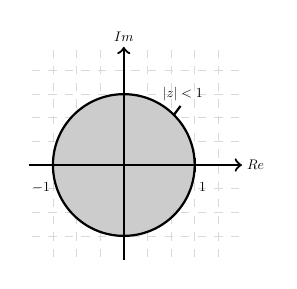
\begin{tikzpicture}[thick,scale=0.3, every node/.style={scale=0.5}]
\draw[help lines, color=gray!30, dashed] (-3.9,-3.9) grid (4.9,4.9);
\draw (2.12,2.12) -- (2.4,2.5);
 \fill[gray!40,even odd rule, dashed] (0,0) circle (3cm);
   \draw (0, 0) circle (3cm) node[above,xshift=1.5cm,yshift=1.5cm]{$|z|<1$};
\draw[thick] (3,-0.3) -- (3,0.3) node[below,xshift=0.2cm,yshift=-0.5cm]{$1$};
\draw[->, thick] (-4,0)--(5,0) node[right]{$Re$};
\draw[->, thick] (0,-4)--(0,5) node[above]{$Im$};
\draw[thick] (-3,-0.3) -- (-3,0.3) node[below,xshift=-0.3cm,yshift=-0.5cm]{$-1$};
\end{tikzpicture}
\end{center}
\end{solution}
\newpage

\begin{problem} $\,$
How many zeros of $p(z)=z^4+z^3+4z^2+2z+7$ lie in the right half plane $\{\re(z)>0\}$?
\end{problem}


\begin{solution}$\,$
First, we check how many times $p$ wraps the imaginary axis (the boundary of the region in question) around the origin.

\begin{align*}
    p(iy)&=(iy)^4+(iy)^3+4(iy)^2+2(iy)+7\\
    &=y^4-iy^3-4y^2+2iy+7\\
    &=y^4-4y^2+7+i(2y-y^3)
\end{align*}

Since $\re(p(iy))'=4y^3-8y$, we can check that $\re(p(iy))$ has minimums at $\pm\sqrt{2}$. Since $y\in\mathbb{R}$ and $\re(p(i\sqrt{2}))=4-8+7>0$ we have that $p(iy)$ always has positive real part and so does not wrap around the origin.

Now, we check how many times $p$ wraps a large circle around the origin. Let $z=Re^{i\theta}$ for $\theta\in[-\frac{\pi}{2},\frac{\pi}{2}]$.

Then $\arg(p(Re^{i\theta}))=\arg(\frac{1}{R^4}p(Re^{i\theta}))$ since multiplying by positive real constants does not change the argument.

However, $$\lim_{R\to\infty}\frac{1}{R^4}p(Re^{i\theta})=\lim_{R\to\infty}e^{4i\theta}+\frac{e^{3i\theta}}{R}+\frac{4e^{2i\theta}}{R^2}+\frac{2e^{i\theta}}{R^3}+\frac{7}{R^4}=e^{4i\theta}.$$

Since $\theta\in[-\frac{\pi}{2},\frac{\pi}{2}]$, $4\theta\in[-2\pi,2\pi]$. Namely, the total change in argument of $p(z)$ is $4\pi$ which implies that $p(Re^{i\theta})$ wraps very large circles around the origin twice.

Therefore, there are \boxed{2} zeros of $p$ in the right-half plane.
\end{solution}
\newpage

\begin{problem} $\,$
Let $f$ be analytic in the unit disk $D=\{|z|<1\}$ and continuous on its closure $\overline{D}$. Show that if $f$ is real valued on the boundary $\partial D=\{|z|=1\}$ then $f$ must be constant.
\end{problem}


\begin{solution}$\,$
Write $f=u+iv$. Since $v$ is harmonic, the maximum and minimum principle states that $v$ must attain both its maximum and minimum on the boundary of any simply connected set.

Therefore, since $f(z)\in\mathbb{R}$ for all $|z|=1$, $v$ is identically $0$ on the boundary of the $\mathbb{D}$ the unit disk.

Thus, $v$ is identically $0$.

Therefore, $f(z)=u(z)\in\mathbb{R}$.

Since $f$ is analytic, Cauchy-Riemann states that $$u_x=v_y=0\qquad\text{ and }\qquad u_y=-v_x=0$$ so $f(z)=u(z)=c$ for some real constant $c$.
\end{solution}
\newpage





\begin{problem} $\,$
By consideration of $\int e^{z+\frac{1}{z}}dz$, or otherwise, show that $$\frac{1}{2\pi}\int_0^{2\pi}e^{2\cos\theta}\cos\theta d\theta=1+\frac{1}{2!}+\frac{1}{2!3!}+\frac{1}{3!4!}+\cdots$$
\end{problem}


\begin{solution}$\,$
Using the hint, we note that $$\int_{|z|=1}e^{z+\frac{1}{z}}dz=\int_0^{2\pi}e^{e^{i\theta}+e^{-i\theta}}ie^{i\theta}d\theta=\int_0^{2\pi}e^{2\cos\theta}i(\cos\theta+i\sin\theta)d\theta.$$

Therefore, \begin{align*}
  \frac{1}{2\pi}\int_0^{2\pi}e^{2\cos\theta}\cos\theta d\theta&=\frac{1}{2\pi i}\int_{|z|=1}e^{z+1/z}dz-\frac{1}{2\pi}\int_0^{2\pi}e^{2\cos\theta}\sin\theta d\theta\\
  &=\frac{1}{2\pi i}\int_{|z|=1}e^{z+1/z}dz+\frac{1}{2\pi}\int_1^1e^{2u}du\qquad u=\cos\theta\\
  &=\frac{1}{2\pi i}\int_{|z|=1}e^{z+1/z}dz\\
  &=\frac{1}{2\pi i}\int_{|z|=1}\sum_{n=0}^\infty\frac{\left(z+\frac{1}{z}\right)^n}{n!}dz\\
  &=\frac{1}{2\pi i}\int_{|z|=1}\sum_{n=0}^\infty\frac{(z^2+1)^n}{z^nn!}dz\\
  &=\sum_{n=0}^\infty\frac{1}{n!}\frac{1}{2\pi i}\int_{|z|=1}\frac{(z^2+1)^n}{z^n}dz\\
  &=\sum_{n=1}^\infty\frac{1}{n!}\frac{1}{(n-1)!}\frac{d^{n-1}}{dz^{n-1}}(z^2+1)^n\big|_{z=0}
\end{align*}
At this point, it is merely a matter of plugging in the first $8$ values of $n$ to obtain the final answer.

It is helpful to note that $$(z^2+1)^n=\sum_{k=0}^n\binom{n}{k}(z^2)^k1^{n-k}=\sum_{k=0}^n\frac{n!}{k!(n-k)!}z^2k.$$

Thus,

\boxed{n=1} $1+z^2\big|_{z=0}=1$

\boxed{n=2} $1+2z^2+z^4$ so the first derivative is $0$ at $0$.

and so forth...
\end{solution}


\end{document}
